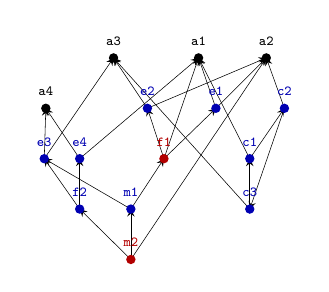
\begin{tikzpicture}[v/.style={circle, fill, inner sep=0.5pt},
  arr/.style={->, >=stealth, very thin}]
  \tikzset{s0/.style={circle, fill=black, inner sep=1.2pt}}
  \tikzset{s1/.style={circle, fill=blue!70!black, inner sep=1.2pt}}
  \tikzset{s2/.style={circle, fill=red!70!black, inner sep=1.2pt}}
  % e1: ref=[a1, a2]
  \draw[arr] (2.43,2.04) -- (2.21,2.68);
  \draw[arr] (2.43,2.04) -- (3.07,2.68);
  % e2: ref=[a2, a3]
  \draw[arr] (1.56,2.04) -- (3.07,2.68);
  \draw[arr] (1.56,2.04) -- (1.13,2.68);
  % e3: ref=[a3, a4]
  \draw[arr] (0.25,1.40) -- (1.13,2.68);
  \draw[arr] (0.25,1.40) -- (0.27,2.04);
  % e4: ref=[a4, a1]
  \draw[arr] (0.70,1.40) -- (0.27,2.04);
  \draw[arr] (0.70,1.40) -- (2.21,2.68);
  % f1: ref=[a1, e1, e2]
  \draw[arr] (1.77,1.40) -- (2.21,2.68);
  \draw[arr] (1.77,1.40) -- (2.43,2.04);
  \draw[arr] (1.77,1.40) -- (1.56,2.04);
  % f2: ref=[e3, e4]
  \draw[arr] (0.70,0.76) -- (0.25,1.40);
  \draw[arr] (0.70,0.76) -- (0.70,1.40);
  % m1: ref=[f1, e3]
  \draw[arr] (1.35,0.76) -- (1.77,1.40);
  \draw[arr] (1.35,0.76) -- (0.25,1.40);
  % m2: ref=[m1, f2, a2]
  \draw[arr] (1.35,0.12) -- (1.35,0.76);
  \draw[arr] (1.35,0.12) -- (0.70,0.76);
  \draw[arr] (1.35,0.12) -- (3.07,2.68);
  % c1: ref=[c2, a1]
  \draw[arr] (2.86,1.40) -- (3.30,2.04);
  \draw[arr] (2.86,1.40) -- (2.21,2.68);
  % c2: ref=[c3, a2]
  \draw[arr] (3.30,2.04) -- (2.86,0.76);
  \draw[arr] (3.30,2.04) -- (3.07,2.68);
  % c3: ref=[c1, a3]
  \draw[arr] (2.86,0.76) -- (2.86,1.40);
  \draw[arr] (2.86,0.76) -- (1.13,2.68);
  % Nodes (drawn last so they sit on top of edges)
  \node[s0] (a1) at (2.21,2.68) {};
  \node[font=\tiny, above=1pt, text=black] at (a1) {\texttt{a1}};
  \node[s0] (a2) at (3.07,2.68) {};
  \node[font=\tiny, above=1pt, text=black] at (a2) {\texttt{a2}};
  \node[s0] (a3) at (1.13,2.68) {};
  \node[font=\tiny, above=1pt, text=black] at (a3) {\texttt{a3}};
  \node[s0] (a4) at (0.27,2.04) {};
  \node[font=\tiny, above=1pt, text=black] at (a4) {\texttt{a4}};
  \node[s1] (e1) at (2.43,2.04) {};
  \node[font=\tiny, above=1pt, text=blue!70!black] at (e1) {\texttt{e1}};
  \node[s1] (e2) at (1.56,2.04) {};
  \node[font=\tiny, above=1pt, text=blue!70!black] at (e2) {\texttt{e2}};
  \node[s1] (e3) at (0.25,1.40) {};
  \node[font=\tiny, above=1pt, text=blue!70!black] at (e3) {\texttt{e3}};
  \node[s1] (e4) at (0.70,1.40) {};
  \node[font=\tiny, above=1pt, text=blue!70!black] at (e4) {\texttt{e4}};
  \node[s2] (f1) at (1.77,1.40) {};
  \node[font=\tiny, above=1pt, text=red!70!black] at (f1) {\texttt{f1}};
  \node[s1] (f2) at (0.70,0.76) {};
  \node[font=\tiny, above=1pt, text=blue!70!black] at (f2) {\texttt{f2}};
  \node[s1] (m1) at (1.35,0.76) {};
  \node[font=\tiny, above=1pt, text=blue!70!black] at (m1) {\texttt{m1}};
  \node[s2] (m2) at (1.35,0.12) {};
  \node[font=\tiny, above=1pt, text=red!70!black] at (m2) {\texttt{m2}};
  \node[s1] (c1) at (2.86,1.40) {};
  \node[font=\tiny, above=1pt, text=blue!70!black] at (c1) {\texttt{c1}};
  \node[s1] (c2) at (3.30,2.04) {};
  \node[font=\tiny, above=1pt, text=blue!70!black] at (c2) {\texttt{c2}};
  \node[s1] (c3) at (2.86,0.76) {};
  \node[font=\tiny, above=1pt, text=blue!70!black] at (c3) {\texttt{c3}};
\end{tikzpicture}